\section{Central forces}
\subsection{Basic definitions}



\subsubsection*{Conditions for a central force}
$\vec{F}_{12}=f(|\vec{r}_{1}-\vec{r}_{2}|)\frac{\vec{r}_{1}-\vec{r}_{2}}{|\vec{r}_{1}-\vec{r}_{2}|}\then \vec{F}(\vec{r})=\mu\ddot{\vec{r}}=f(r)\frac{\vec{r}}{r}$, in such case the following equations hold: $\ddot{r}-r\dot{\theta}^{2}=\frac{f(r)}{\mu},\ r\ddot{\theta}+2\dot{r}\dot{\theta}=0$



\subsection{Conserved quantities}
$\vec{L}=\mu\vec{r}\times\dotv{r}=\mu r^{2}\dot{\theta}\vec{e}_{z},\ |\vec{L}|=L_{z}=\dot{\theta}r^{2}\mu>0$\\
$E=\frac{1}{2}\mu\dot{r}^{2}+U(r)=\frac{L^{2}}{2\mu}(u'^{2}+u^{2})+V(\frac{1}{u})$\\
\begin{wrapfigure}[0]{r}[0pt]{0cm}
 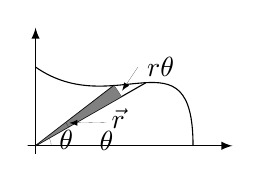
\begin{tikzpicture}
\clip(-0.1,-0.1) rectangle (2.5,1.5);
\draw[-latex] (0,-0.2) -- (0,1.5);
                        \draw[-latex] (-0.2,0) -- (2.5,0);
                        \draw (0,1) .. controls (1,0.3) and (2,1.5) .. (2,0);
                        \draw (0,0) -- (1.4,0.8) node[near end,below]{$\vec{r}$};
                        \draw (0,0) -- (1,0.77);
                        \draw[line width=0.01mm,-latex] (1.3,1) -- (1.1,0.7) node[at start,right]{$r \dd{\theta}$};
                        \fill[line width=0.01mm,gray,draw=black] (0,0) -- (1.092,0.624) arc (30:37:1.39) -- (0,0);
                        \draw[line width=0.01mm,] (0.2,0) arc (0:29:0.2) node[near end,right]{$\theta$};
                        \draw[line width=0.01mm,] (0.42,0.24) arc (30:37:0.484);
                        \draw[line width=0.01mm,-latex] (0.9,0.3) -- (0.43,0.29) node[at start, below]{$\dd{\theta}$};
                        \end{tikzpicture}
                        \end{wrapfigure}



\subsubsection*{Law of areas}
 $A(\theta)=\frac{1}{2}\scaleint{5ex}^{\theta}_{\theta_{0}} r^{2}(\alpha) \dd{\alpha},\ $\\
 $\dot{A}=\frac{\dd{A}}{\dd{\theta}}\dot{\theta}=\frac{1}{2}r^{2}\dot{\theta}=\frac{L}{2\mu}\in \R$


\subsection{Important equations}
\subsubsection*{Binet's eqn.}
$f(r)=-\frac{L^{2}}{\mu r^{2}}(u''+u)$




\subsubsection*{Other equations}
$U(r)=V(r)+\frac{L^{2}}{2\mu r^{2}},\ -\partials{}{\vec{r}}\Big(\frac{L^{2}}{2\mu r^{2}}\Big)=\frac{\mu v_{\theta}^{2}}{r}\vec{e}_{r}$\\
$t=\pm \sqrt{\frac{\mu}{2}}\scaleint{5ex}_{r_{1}}^{r_{2}}\frac{\dd{r}}{\sqrt{E-U(r)}}=\frac{\mu}{L}\scaleint{5ex}_{r_{1}}^{r_{2}}r^{2}(\theta)\dd{\theta},$\\
$\theta=\frac{L}{\mu}\scaleint{5ex}_{t_{1}}^{t_{2}}\frac{\dd{t}}{r^{2}(t)}=\pm\frac{L}{\sqrt{2\mu}}\scaleint{5ex}^{\frac{1}{r}}\frac{\dd{u}}{\sqrt{E-U(\frac{1}{u})}},$\\
$\tau_{r}=\sqrt{2\mu}\scaleint{5ex}_{r_{1}}^{r_{2}}=\frac{\dd{r}}{\sqrt{E-U(r)}},\ $
$\Delta{\theta}=\sqrt{\frac{2L^{2}}{\mu}}\scaleint{5ex}_{\frac{1}{r_{2}}}^{\frac{1}{r_{1}}}=\frac{\dd{u}}{\sqrt{E-U(\frac{1}{u})}},$\\
$\text{ An orbit is periodic $\iff \Delta\theta=q\pi,\ q\in\Q$}.$\\
$A_{T}=\pi r^{2}=\pi ab=\dot{A}\cdot\tau=\frac{L}{2\mu}\tau,$\\
$v=\frac{L}{\mu}\sqrt{u'^{2}+u^{2}}$


\subsection{Kepler's potential}



\subsubsection*{Force field and Binet's eqn.}
$\vec{F}(\vec{r})=-\frac{k}{r^{2}}\vec{e}_{r},\ V(r)=-\frac{k}{r},\ \ddot{\vec{r}}=-GM\frac{\vec{r}}{r^3}$,\ 
$u''+u=\frac{\mu k}{L^{2}}$



\subsubsection*{Equation of trajectory and its clasifications}
$u=\frac{\mu k}{L^{2}}(1+e\cos(\theta-\theta_{0})),\ e,\theta_{0}\in\R.$\\
$r=\frac{\alpha}{1+e\cos(\theta)},\ \alpha\equiv\frac{L^{2}}{\mu k},\ e=\sqrt{1+\frac{2EL^{2}}{\mu k^{2}}}\geq0$\\
$
\left\{
\begin{aligned}
e&>1     &    &\iff     &   E&>0  &  &\Rightarrow   &   &\text{hyperbola}\\
e&=1     &   &\iff  &   E&=0  &  &\Rightarrow   &   &\text{parabola}\\
e&\in(0,1)   &   &\iff  &   E&\in(-\frac{\mu k^{2}}{2L^{2}},0)  &  &\Rightarrow   &   &\text{ellipse}\\
e&=0     &    &\iff     &   E&=-\frac{\mu k^{2}}{2L^{2}}    &   &\Rightarrow   &   &\text{circle}
\end{aligned}
\right.$


\subsection{Planetary motion}
\subsubsection*{Study of ellipses}
                            $\vec{C}\equiv\{(1-e^{2})(x+\frac{\alpha e}{1-e^{2}})^{2}+y^{2}=\frac{\alpha^{2}}{1-e^{2}}\}$\\
                            $a=\frac{\alpha}{1-e^{2}},\ b=\frac{\alpha}{\sqrt{1-e^{2}}},\ $$c=\varepsilon a=ea,\ e=\varepsilon,$\hfill\\
                            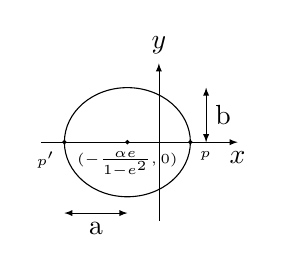
\begin{tikzpicture}[{baseline=(current bounding box.north)}]
                            \draw[line width=0.01mm,-latex] (-1.5,0) -- (1,0) node[at end,below]{$x$};
                            \draw[line width=0.01mm,-latex] (0,-1) -- (0,1) node[at end,above]{$y$};
                            \draw (-0.4,0) ellipse (0.8 and 0.693);
                            \draw[line width=0.01mm,latex-latex] (0.6,0) -- (0.6,0.693) node[midway,right]{b};
                            \draw[line width=0.01mm,latex-latex] (-0.4,-0.9) -- (-1.2,-0.9) node[midway,below]{a};
                            \filldraw[black] (-0.4,0) circle (0.02) node[below]{\tiny{$(-\frac{\alpha e}{1-e^{2}},0)$}};
                            \filldraw[black] (0.4,0) circle (0.02) node[anchor=north west]{\tiny{$p$}};
                            \filldraw[black] (-1.2,0) circle (0.02) node[anchor=north east]{\tiny{$p'$}};
                            \end{tikzpicture}
                            \\
$E=-\frac{k}{2a},\ \langle r\rangle=\Big(1+\frac{e^{2}}{2}\Big)a,$\\
$\tau=2\pi\sqrt{\frac{\mu}{k}}a^{3/2}=\pi k\sqrt{\frac{\mu}{2}}|E|^{-3/2}
                                =\frac{2\pi a^{3/2}}{\sqrt{GM}}\simeq\frac{2\pi a^{3/2}}{\sqrt{GM_{\odot}}}$\\
$p=\frac{\alpha}{1+e}=a(1-e),\ p'=\frac{\alpha}{1-e}=a(1+e),$\\
$v^{2}=\frac{k^{2}}{L^{2}}(1+e^{2}+2e\cos\theta)\then \left\{
\begin{aligned}
v_{p}&=\frac{k}{L}(1+e)=\sqrt{\frac{k}{\mu p}(1+e)}\\
v_{p'}&=\frac{k}{L}(1-e)=\sqrt{\frac{k}{\mu p'}(1-e)}
\end{aligned}
\right.$










